\section{Tema 2: Kvantebrønner}
\label{tema2}

\begin{table}[!htb]
    \centering
    \caption{Samtale punkter for tema 2}
    \begin{tabular}{|c|c|c|r|}
      \hline
      1 & Bundne og spredende tilstander &  \autoref{sec:tema2_1} & \cellcolor{blue}\quad\quad \\
      \hline 
      2 & Uendelig dyp kvantebrønn i 1D & \autoref{sec:tema2_2} & \cellcolor{green} \\
      \hline
      3 & Målepostulatet & \autoref{sec:tema2_3} & \cellcolor{green} \\
      \hline
      4 & Endelig kvantebrønn & \autoref{sec:tema2_4} & \cellcolor{blue} \\
      \hline 
      5 & Tunnellering & \autoref{sec:tema2_5} & \cellcolor{green} \\
      \hline
      6 & Pertubasjonsteori & \autoref{sec:tema2_6} & \cellcolor{green} \\ 
      \hline
    \end{tabular}
    \label{tab:samtalePunkt_tema1}
\end{table}

\subsection{Bundne og spredende tilstander}
\label{sec:tema2_1}
Bunnede og spredde tilstander er greit å ha en intuisjon om, kvantemekanikken er i hovedsak veldig lik den klassiske mekanikken, men med noen små avvik som vi skal gå inn på senere i \autoref{tema2}.

Enkelt forklart er bundet tilstander de tilstandene som binder et objekt. Se for deg du er i en berg og dalbane, bestående av en loop, start er bunnen av loopen, og det er også slutten. Si man kommer opp kvarte sirkelen. Bremsene slutter å funke og man sklir nedover igjen til start, i et system med energibevaring vil man ende like høy oppe på andre siden av loopen. Du er nå i en bundet tilstant, der den klassiske vendepunktet er punktet der du ikke har noe kinetiske energi, kun potensiell energi. \autoref{fig:bundet} er ikke berg og dalbane eksempelet, men med en generisk vogn.

\begin{figure}[!htb]
    \centering
    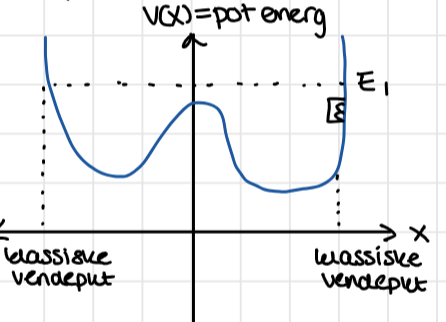
\includegraphics[scale=1]{Bilder/SamtaleTema2/Bundet og spredde/bundneTilstander.png}
    \caption{Systemet viser en vogn som er i en bundet tilstand}
    \label{fig:bundet}
\end{figure}

Vi kan spille videre på berg og dalbane eksempelet, se for deg en annen bane nå, der man kommer på flatmark i høy hastighet, foran deg er det en høyde. Den kinetiske energien til systemet gjør at man fyker rett over. Dette er et eksempel på en spredt tilstand, dersom du ikke kommer over vil du falle ned igjen på samme side, og forsvinne vekk fra høyden.

\begin{figure}[!htb]
    \centering
    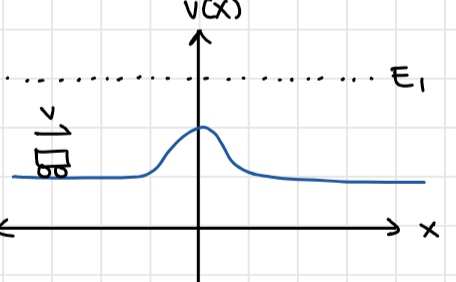
\includegraphics{Bilder/SamtaleTema2/Bundet og spredde/SpredteTilstander.png}
    \caption{Vogn på vei til en høyde, vognen er ikke låst til et område på x-aksen.}
    \label{fig:spredt}
\end{figure}
\newpage
\autoref{fig:kombinert} viser en figur der begge tilstandene oppstår, så avhengig av initial betingelsene kan en vogn ende opp med å bli bundet eller spred.

\begin{figure}[!htb]
    \centering
    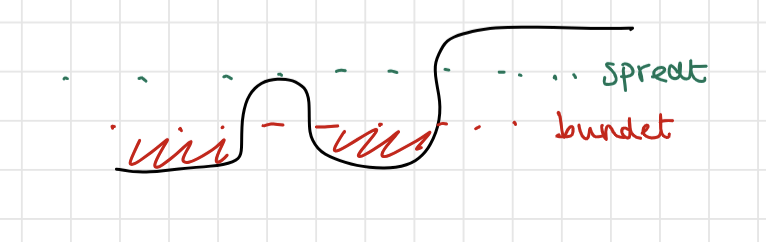
\includegraphics{Bilder/SamtaleTema2/Bundet og spredde/KombinerteTilstander.png}
    \caption{}
    \label{fig:kombinert}
\end{figure}

I kvantemekanikken oppfører en kvantepartikkel seg som det klassiske tilfellet, men ved de klassiske vendepunktene skjer det uventede. Vi starter med å se på SL for en kvantepartikkel i en potensiale.

\begin{equation}
    \label{eq:spredKvantte}
    \begin{split}
     E\psi(x)  &= -\frac{\hbar^2}{2m}\frac{\partial^2 \psi(x)}{\partial x} + V(x)\psi(x)\\
    \psi''(x) &= -\frac{2m(E-V(x))}{\hbar^2}\psi(x)\\
    \psi''(x) &= \alpha\psi(x)
    \end{split}
\end{equation}

vi kaller uttrykket foran $\psi(x)$ for $\alpha$. Vi på energien til partikkelen, dersom den er større enn potensialet $V(x)$ vil $\alpha < 0$ dette fører til trigonometriske løsninger, videre hvis energien $E < V(x)$ blir løsningen eksponentiell siden $\alpha > 0$.

I en uendelig kvantebrønn (se \autoref{sec:tema2_2}), kan man kun ha bundne tilstander, da det er ufysisk for en kvantepartikkel å være i et uendelig potensiale. I en endelig kvantebrønn er det ikke null sannsynlighet for at partikkelen eksisterer utenfor de klassiske grensene (se \autoref{sec:tema2_4}).

\renewcommand{\arraystretch}{1.5}% Vertically stretch tabular constructions
\noindent
\begin{tabularx}{\textwidth}{
    @{\hspace{1.5em}}% Space for left bullet
    >{\leavevmode\llap{\textbullet~}\raggedright}% Left bullet + formatting of column
    X% Left column specification
    @{\quad\hspace{1.5em}}% Space between columns + right bullet space
    >{\leavevmode\llap{\textbullet~}\raggedright\arraybackslash}% Right bullet + formatting of column
    X% Right column specification
    @{}% No column space on right
  }
  \toprule
  \multicolumn{1}{X}{\centering\bfseries Bundne Tilstander} &
    \multicolumn{1}{X}{\centering\bfseries Spredde Tilstander} \\
  \midrule
    Avgrenset i rom  & 
    Ikke avgrenset i rom  \\
    Normaliserbare ($\psi$ går mot 0 ved $\pm \infty$) & ikke normaliserbare ( bølgefunksjonen har ikke definert areal under grafen) \\
    Kvantiserte av randbetingelser (randbetingelsene begrenser energinivåene som er tilgjengelige for systemet, og disse energinivåene er kvantisert) & 
    Ikke kvantiserte (kontinuerlig spektrum, alle energinivåer lov) \\
    De antar bare diskrete bestemte verdier & - \\
  \bottomrule
\end{tabularx}

\begin{figure}[!htb]
    \centering
    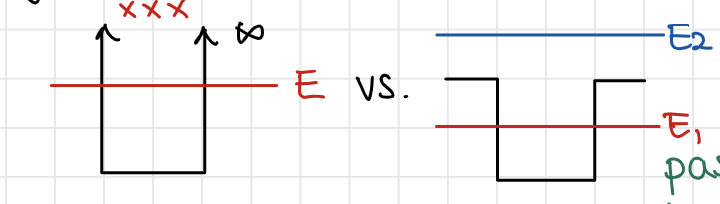
\includegraphics{Bilder/SamtaleTema2/Bundet og spredde/endeligvsuendelig.png}
    \caption{Røde kryssene over uendelig kvantebrønn indikerer at det ikke er mulig å ha energi utenfor brønnen, men dette er mulig for den endelige brønnen.}
    \label{fig:endeligVSuendelig}
\end{figure}

\newpage
\subsection{Uendelig dyp kvantebrønn i 1D}
\label{sec:tema2_2}
\subsubsection{Fri partikkel}
Før vi kan se på en uendeig dyp kvantebrønn, kan vi se på en fri partikkel. Partikkelen er ikke påvirket av et potensial, så all energien til partikkelen er ''bakt'' inn i bevegelsesmengden. I \autoref{eq:shrodinger_freeparticle} har vi allerrede sett uttrykket og seksjonen går litt inn på utledningen. Vi vil gjerne se på et plot som sammenligner energien og bølgetallet $k$, ved å forenkle ligning \ref{eq:shrodinger_freeparticle} får vi 

\begin{equation}
    \label{eq:free_part_simplified}
    \frac{\hbar^2}{2m} \frac{\partial^2 \psi(x)}{\partial x^2} + E\psi(x) = 0,
\end{equation}

Løsningen til ligning \ref{eq:free_part_simplified} er en funksjon som også er egentilstanden til både energi og bevegelsesmengde.

\begin{equation}
\label{eq:solPsi_freeparticle}
    \psi(x) = Ae^{ikx}
\end{equation}

Setter vi ligning \ref{eq:solPsi_freeparticle} inn i ligning \ref{eq:free_part_simplified} får vi

\begin{equation}
    \label{eq:freeLastEq}
    -\frac{\hbar^2k^2}{2m}\psi(x) + E\psi(x) = 0,
\end{equation}

Vi sitter igjen med at det kun er én ikke triviell løsning til ligning \ref{eq:freeLastEq}. \autoref{eq:Evalue_free} viser bevegelsesmengde energien.

\begin{empheq}[box=\tcbhighmath]{align}
    \label{eq:Evalue_free}
    E = \frac{\hbar^2k^2}{2m}
\end{empheq}

Vi ser nå at forholdet mellom energien og bølgetallet er kvadratisk. \autoref{fig:parabola} viser en parabel. Denne funksjonen er kontinuerlig, Energien i dette tilfellet er ikke kvantisert.

\begin{figure}[!htb]
    \centering
    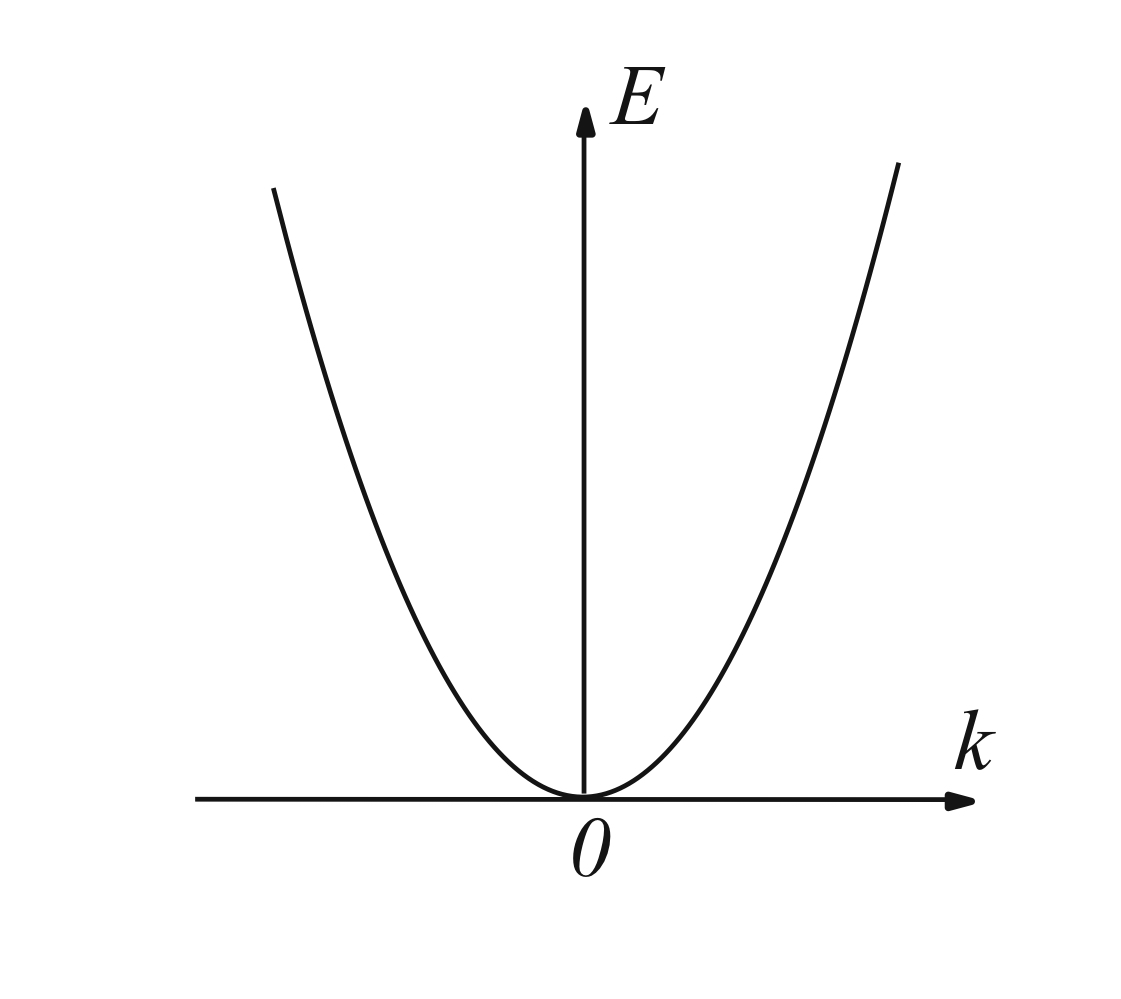
\includegraphics[scale=0.25]{Bilder/SamtaleTema2/FreeParticleEnergy.jpg}
    \caption{Energi - bevegelsesmengde forholdet for en fri partikkel}
    \label{fig:parabola}
\end{figure}

Intervallet partikkelen vil kunne bevege seg på er $[-L,L]$, der $L$ går mot $\infty$.

\subsubsection{Uendelig dyp kvantebrønn 1D}
Ved å begrense partikkelen og innføre grensebetingelser får vi en litt annen oppførsel. Vi sier at partikkelen kan bevege seg mellom $[0,a]$ der $a$ har en definert verdi. Potensialet til brønnen kan representeres som

\begin{equation}
\label{eq:potInfinite}
V(x) = \left\{
        \begin{array}{ll}
            -\infty & \quad x \leq 0 \\
            0 & \quad 0 \leq x \geq a \\
            \infty & \quad x \geq a
        \end{array}
    \right.
\end{equation}

Ved å ta i bruk funksjonen for spenningen fra ligning \ref{eq:potInfinite} kan vi skissere opp systemet, dette er visualisert i figur \ref{fig:1DInfWell}

\begin{figure}[!htb]
    \centering
    \includegraphics[scale=0.2]{Bilder/SamtaleTema2/1DUendeligBrønn.jpg}
    \caption{Potensiell energi for en 1D box.}
    \label{fig:1DInfWell}
\end{figure}

Konsekvensen av å sette potensialet lik $\infty$ utenfor den en dimensjonale boksen gjør at bølgefunksjonen $\psi(x)$ vil være null. Fordi en partikkel ikke kan inneha uendelig energi. Dette fører også til at vi får grensebetingelser på systemet vårt, representert med ligning \ref{eq:randBetingelser1D}

\begin{equation}
    \label{eq:randBetingelser1D}
    \psi(0) = \psi(a) = 0
\end{equation}

\autoref{eq:solPsi_freeparticle} er en løsning for dette systemet også, men det er gunstig å skrive det om til sinus og cosinus. 

\begin{equation}
    \psi(x) = Asin(kx) + Bcos(kx)
\end{equation}

løser vi med hensyn på randbetingelsene får vi at $B=0$ og $Asin(ka)=0$. Siden bølgefunksjonen ikke kan være null i hele rommet, må det bety at 

\begin{equation}
    ka = n\pi \implies k_n = n\frac{\pi}{a},
\end{equation}

Vi ser nå at i motsetning til fri partikkel, kan ikke bølgenummeret k være en kontinuerlig funksjon, altså energinivåene er kvantiserte. Energi uttrykket kan skrives som 

\begin{empheq}[box=\tcbhighmath]{align}
    \label{eq:1D-particleEnergy}
    E_n = \frac{\hbar^2 \pi^2 n^2}{2ma^2}
\end{empheq}

For å finne normaliseringskonstanten er det bare å sette inn i ligning \ref{eq:normalisering}, og framgangsmåten er relativt intuitiv.

\subsection{Målepostulatet}
\label{sec:tema2_3}
Målepostulatet i kvantemekanikken sier at når vi gjør en måling av en kvantepartikkel (f.eks posisjon eller spinn), får vi et bestemt resultat med en viss sannsynlighet. 

For at en løsning til SL skal kunne representere en partikkel må denne løsningen være ''normaliserbar''. Normalisering er bevart over tid dersom $\hat{H}$ er en Hermittisk operator. En Hermittisk operator er en operator som oppfyller ligning \ref{eq:hermit}

\begin{equation}
    \label{eq:hermit}
    \int \Psi_1^*\hat{H}\Psi_2 = \int \bigl(\hat{H}\Psi_1\bigl)^*\Psi_2
\end{equation}

Dette er også sant for $\Psi_2^*\Psi_1$ og $\Psi_1^*\Psi_1$. Hermittiske operatorer har alltid reelle egenverdier

\begin{equation}
    \hat{H}\psi = E\psi
\end{equation}
Her er $E$ en egenverdi og $\psi$ er en egenfunksjon. Så alle operatorer som produserer reelle egenverdier er Hermittiske.

Hermittiske operatorer har et komplett sett av ortonormale egenfunksjoner. Funksjonen står vinkelrett på hverandre dersom det indreproduktet er lik null. For bølgefunksjonen får vi

\begin{equation}
\label{eq:hemittisk}
\int \Psi_m^*\Psi_n = \delta_{mn} \left\{
        \begin{array}{ll}
            0 & \quad m \neq n \\
            1 & \quad m = n 
        \end{array}
    \right.
\end{equation}

Fra det komplette settet kan vi representere en hver relevant bølgefunksjon ved superposisjon

\begin{equation}
    \label{eq:superpos}
    \psi(x) = \alpha_1\psi_1{x} + \alpha_2\psi_2{x} + \alpha_3\psi_3{x} + ...
\end{equation}

$\alpha_i$ er i dette tilfellet en sannsynlighetsvekt, så dersom vi skulle målt en av bølgene må en av disse velges ved kollapsen av bølgefunksjonen. Dersom vi har en vilkårlig Hermittisk operator vi kaller $\hat{Q}$, og anvender denne på $\psi$ vil vi \textbf{kun} måle en av egenverdiene. og sannsynligheten for å måle $q_i$ er

\begin{equation}
    p_i = |\alpha_i|^2 = \int \psi_i^*\psi dx
\end{equation}

Etter utfallet av $q_i$ er målt, blir tilstanden til systemet $\psi(x)=\psi_i(x)$. Vi sier med det at bølgefunksjonen har kollapset. Dersom det blir gjort en måling rett etter, vil resultatet være det samme. Men etter tid vil bølgefunksjonen inneha et likt ''uordnet'' system.

\subsection{Endelig kvantebrønn}
\label{sec:tema2_4}
\autoref{fig:finiteSquare} viser en endelig kvantebrønn, hvis en partikkel har total energi som er større enn $V_0$ vil vi ha en spredende tilstand, vi er ikke interessert i disse i dette kapitellet. Vi kan dele systemet inn i tre soner, \rom{1} er alt til venstre for $-\frac{a}{2}$ og \rom{3} er alt til høyre for $\frac{a}{2}$. Region \rom{2} er området i mellom \rom{1} og \rom{3}.

\begin{figure}[!htb]
    \centering 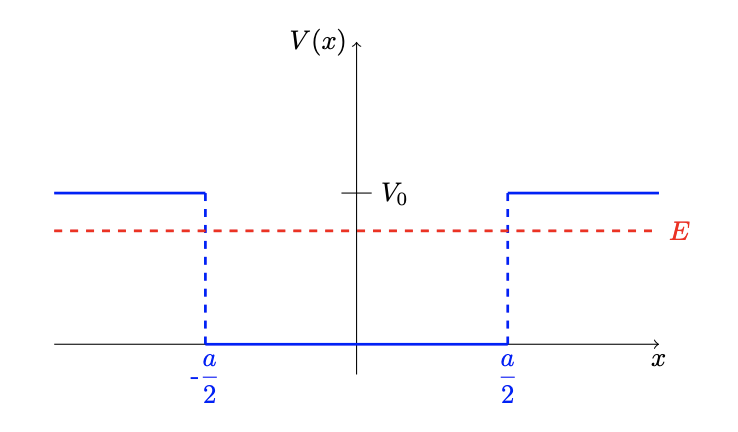
\includegraphics[scale=1]{Bilder/SamtaleTema2/endeligKvanteBrønn/FiniteSquare.png}
    \put(-300,80){\rom{1}}
    \put(-190,80){\rom{2}}
    \put(-80,80){\rom{3}}
    \caption{Endelig kvantebrønn, fortsatt 1D (partikkelen lever på x-aksen)}
    \label{fig:finiteSquare}
\end{figure}

sone \rom{1} og \rom{3} er klassiske forbudte områder, men en kvantepartikkel kan finne på å ende opp der. I region \rom{2} er 
$\alpha < 0$ (samme $\alpha$ fra ligning \ref{eq:spredKvantte}, vi får trigonometriske løsninger. Region \rom{1} og \rom{3} vil ha $\alpha > 0$ som gir oss eksponentielle løsninger.

\begin{figure}[!htb]
    \centering
    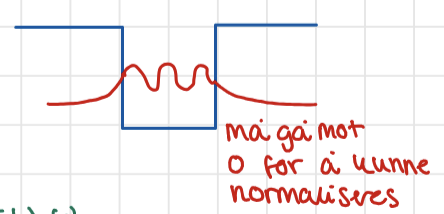
\includegraphics[scale=1]{Bilder/SamtaleTema2/endeligKvanteBrønn/nrmali.png}
    \caption{Viser oss at sannsynligheten for å finne en bølge utenfor det klassiske forbudte området er større enn null}
    \label{fig:normalComment}
\end{figure}

Viktige kriterier for løsningen av problemmet endelig kvantebrønn er veldig lik kriteriene for den uendelige kvantebrønnen er randbetingelsene. Men nå har vi også

\begin{equation*}
    \begin{split}
        \psi_{\rom{1}}(-\frac{a}{2}) &= \psi_{\rom{2}}(-\frac{a}{2}) \\
        \psi_{\rom{2}}(\frac{a}{2}) &= \psi_{\rom{3}}(\frac{a}{2}) \\
        \frac{\partial}{\partial x}\psi_{\rom{1}}(-\frac{a}{2}) &= \frac{\partial}{\partial x}\psi_{\rom{2}}(-\frac{a}{2}) \\
        \frac{\partial}{\partial x}\psi_{\rom{2}}(\frac{a}{2}) &= \frac{\partial}{\partial x}\psi_{\rom{3}}(\frac{a}{2}) 
    \end{split}
\end{equation*}

Vi definerer nå variabelen k som 

\begin{equation}
\label{eq:k_endelig}
    k^2 = \frac{2m}{\hbar^2}(V_0-|E|) > 0
\end{equation}

Uttrykket $V_0-|E|$ sier oss noe om ''avstanden'' fra potensial til energi. Innenfor region \rom{2} er den større enn null.

Sette vi inn det vi har til nå i SL får vi at $\psi'' = -k^2\psi$, dette gir sin/cos løsninger, men siden vi har kun har symmetriske løsninger kan vi si at

\begin{equation}
    \psi(x) = ... cos(kx) \quad ; \quad -\frac{a}{2} < x < \frac{a}{2}
\end{equation}

I dette tilfellet dropper vi normaliseringskonstanten. Løsningen for region \rom{3} blir lik som for region \rom{1}. Ved utledning finner vi

\begin{equation}
\label{eq:3}
\begin{split}
    \psi''(x) &= -\frac{2m}{\hbar^2}E\psi(x) \\
    \psi''(x) &= \frac{2m|E|}{\hbar^2}\psi(x) \\
    \psi''(x) &= \kappa^2\psi(x)
\end{split}
\end{equation}

Løser ligningen vi sitter igjen med fra \ref{eq:3}, får vi for $\psi(x)$ to løsninger

\begin{equation}
    \label{eq:sol1_sol3}
    \psi(x) = Ae^{\pm kx}
\end{equation}

\autoref{eq:sol1_sol3} viser oss at ved $x<-\frac{a}{2}$ får vi en positiv eksponent, og for $x>\frac{a}{2}$ får vi en negativ en, så når begge sider går mot uendelig går bølgefunksjonen mot null.

For å gjøre neste delen litt enklere gjør vi om bredden på brønnen til å gå fra $-a$ til $a$, dette gjør noen av uttrykkene litt enklere å jobbe med. 

Vi har nå to bølgetall, $\kappa$ og $k$. De hører til forskjellige regioner. Man kan tolke det som lysbølge som beveger seg  vakuum sammenlignet med i vann. Når den beveger seg i vakuum har bølgen et spesefikt bølgetall, mens når den beveger seg i vann har den et annet. Dette kan sammenlignes med potensialet $V(x)$, når bølgen er utenfor det klassiske området vil potensialet være anerledes, og dermd gir det et annet bølgetall sammenlignet med det som oppstå i brønnen.

\begin{equation}
\label{eq:kappashit}
    \begin{split}
        \kappa^2 + k^2 &= \frac{2mV_0}{\hbar^2} \\
        \kappa^2a^2 + k^2a^2 &= \frac{2mV_0a^2}{\hbar^2}, \quad \zeta = \kappa a,\, \eta = ka \\
        \zeta^2 + \eta^2 &= Z_0^2
    \end{split}
\end{equation}

\autoref{eq:kappashit} viser en ligning som forteller oss om forholdet mellom bølgetallene, på høyre siden sitter vi igjen med et uttrykk som forteller oss om den endelige kvantebrønnen vi ser på. Siden $\zeta> 0$ og $\eta>0$, får vi en kvart sirkel i $\zeta$- og $\eta$-planet.

$\psi$ er kontinuerlig i $x=a$ det gir oss
\begin{equation}
\label{eq:1}
    cos(ka)=Ae^{-\kappa a}
\end{equation}
og $\psi'$ er også kontinuerlig i $x = a$ som gir
\begin{equation}
\label{eq:2}
    ksin(ka) = \kappa Ae^{-\kappa a}
\end{equation}

Både ligning \ref{eq:1} og \ref{eq:2} representerer grensebetingelsene i overgangen mellom region \rom{2} og \rom{3}. Dersom vi deler ligning \ref{eq:1} på ligning \ref{eq:2} får vi

\begin{equation}
\label{eq:even}
    \frac{\rom{2}}{\rom{1}} \, : \,
    ktan(ka) = \kappa \implies \zeta = \eta tan(\eta),
\end{equation}

for den like løsningen, og for den odde løsningen får vi

\begin{equation}
    \label{eq:odd}
    \zeta = -\eta cot(\eta)
\end{equation}

\autoref{fig:losningEndeligGrafisk} 

\begin{figure}[!htb]
    \centering
    \subfloat[\centering Like løsninger fra ligning \ref{eq:even}]{{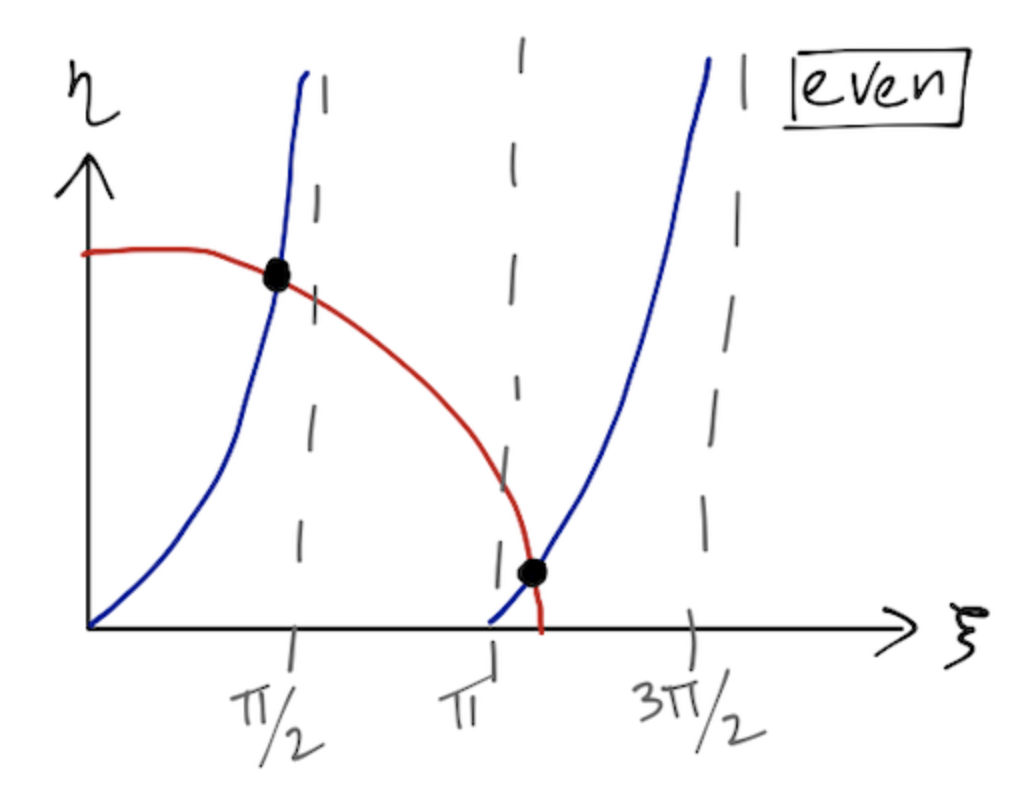
\includegraphics[width=7cm]{Bilder/SamtaleTema2/endeligKvanteBrønn/evenSol.png} }}%
    \qquad
    \subfloat[\centering Odde løsninger fra ligning \ref{eq:odd}]{{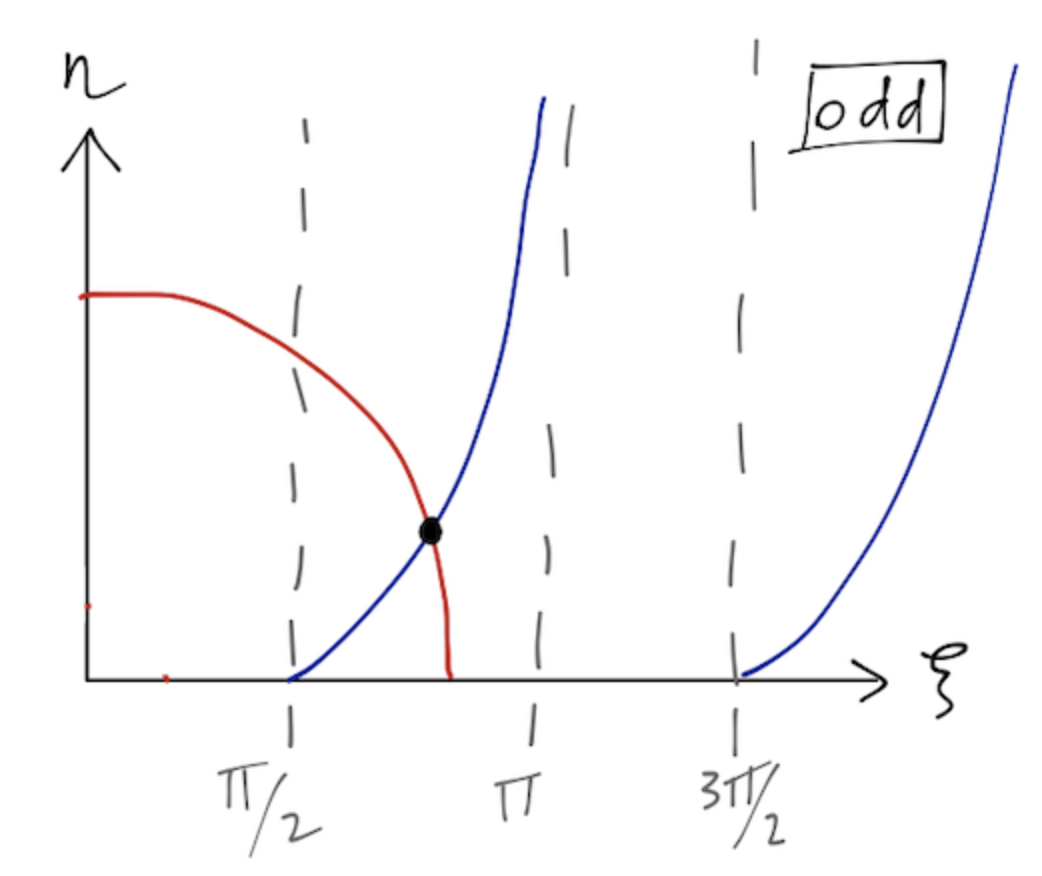
\includegraphics[width=7cm]{Bilder/SamtaleTema2/endeligKvanteBrønn/oddSol.png} }}%
    \caption{2 Figures side by side}%
    \label{fig:losningEndeligGrafisk}%
\end{figure}

NB! aksene her er ikke riktig, $\zeta$ skal være på y-aksen og $\eta$ skal på x-aksen.

Selvom $Z_0$ (radiusen til den røde sirkelen) er liten i.e. brønnen er veldig lite dyp, vil det alltid være plass til minst en bølgefunksjon. 

Tilegg: Potensialet  $V_0$ er det som bestemmer ''dybden'' på den endelige kvantebrønnen. det er derimot energien $E$ som bestemmer hvor ''høyt'' oppe partikkelen kan befinne seg.

\subsection{Tunnellering}
\label{sec:tema2_5}
Tunnellering er et kvantemekaniske fenomen der en partikkel klarer å bevege seg gjennom en barriere av potensiell energi som har en høyere energi enn partikkelens kinetiske energi. Mer som dette i \autoref{tema3}.

\subsection{Pertubasjonsteori}
\label{sec:tema2_6}
Pertubasjonsteori er en systematisk metode for å finne tilnærmede løsninger til perturberte kvantemekaniske system. Kravet for å anvende teorien er at perturabsjonen er ''liten'' og løsninger for det uperturberte systemet er kjent. Det vil si at dersom vi legger en perturbasjone i en uendelig kvantebrønn, kjenner vi allerede løsningen for det uperturberte systemet. Vi kan derfor bruke det som utgangspunkt til å finne løsningen til det perturberte sysemet. 

Det vi ønsker å finne med perturbasjonteori er en Hamiltonian som for det perturberte systemet. En kan se på en perturbasjon som en forstyrrelse i form av et potensial som blir lagt til i systemet. Vi definerer løsningen til det uperturberet systemet som 

\begin{equation}
    \label{eq:solUpert}
    \hat{H}^{(0)}\psi_n^{(0)} = E_n^{(0)}\psi_n^{(0)},
\end{equation}

For det perturberte systemet blir dette 

\begin{equation}
    \label{eq:hamPert}
    \hat{H} = \hat{H}^{(0)} + \hat{u}_{pert}
\end{equation}

Pertubasjonsteori gir oss den totale energien og bølgefunksjonen som en sum av korreksjonsedd. Dersom antall ledd går mot uendelig vil løsningen være riktig, men dette gjelder kun for ikke analytiske systemer. lignende taylor rekker vil det første leddet bære med vekt og leddene sine vekter vil anta ettersom ledd indexen øker.

\begin{equation}
    \label{eq:pertEnergi}
    E_n = E_n^{(0)} + E_n^{(1)} + E_n^{(2)} + ... + E_n^{(m)}
\end{equation}

\begin{equation}
    \label{eq:pertWave}
    \psi_n = \psi_n^{(0)} + \psi_n^{(1)}  + \psi_n^{(2)}+ ... + \psi_n^{(m)} 
\end{equation}

Første ordens korreksjons ledd for $E_n$

\begin{equation}
    E_n^{(1)} = \bra{n^{(0)}} \hat{u}_{pert} \ket{n^{(0)}}
    =
    \int_{-\infty}^{\infty} \psi_n^{(0)*}u_{pert}\psi_n^{(0)}dx
\end{equation}

Den perturberte løsningen inneholder litt høyere energi, dette er fordi tilførselen av et potensial i den endelig kvantebrønnen gjør at det innføres mer krumming i bølgefunksjonen, og energi er proporsjonalt med krumningen til bølgefunksjonen. 

\begin{figure}[!htb]
    \centering
    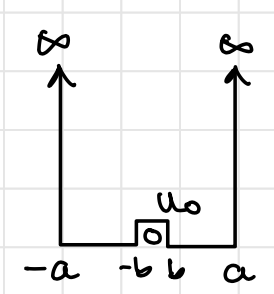
\includegraphics{Bilder/SamtaleTema2/Pertubasjonsteori/pert.png}
    \caption{Endelig kvantebrønn med tilførsel av en perturbasjon lokalisert i midten av brønnen.}
    \label{fig:figPert}
\end{figure}

\newpage